\documentclass[border=6pt]{standalone}
\usepackage{amsmath,amssymb}
\usepackage[dvipsnames]{xcolor}
\usepackage{tikz}
\usetikzlibrary{arrows.meta,calc,positioning}
\definecolor{cvprblue}{rgb}{0.21,0.49,0.74}
\renewcommand{\familydefault}{\sfdefault}
\begin{document}
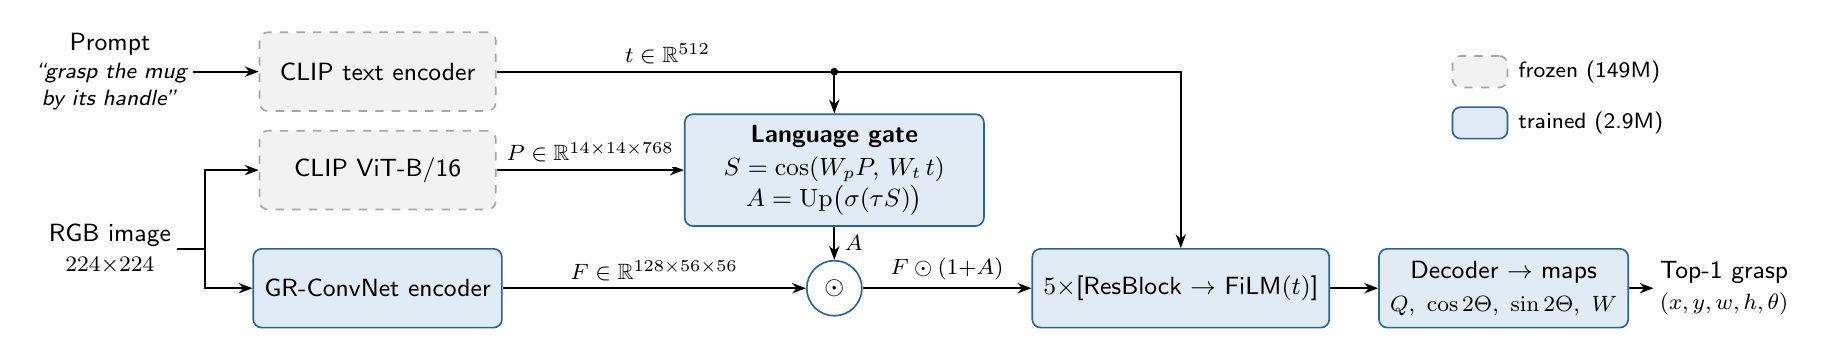
\begin{tikzpicture}[
  font=\sffamily\small, >={Stealth[length=5pt]}, line width=0.6pt,
  blk/.style={draw, rounded corners=3pt, align=center, minimum height=10mm, inner sep=4pt},
  frz/.style={blk, fill=gray!10, dashed, draw=gray!70},
  trn/.style={blk, fill=cvprblue!15, draw=cvprblue!80!black},
  io/.style={align=center, inner sep=2pt},
  lab/.style={font=\sffamily\footnotesize, fill=white, inner sep=1.5pt},
  op/.style={draw=cvprblue!80!black, circle, fill=white, inner sep=1pt, minimum size=7mm}]
  % inputs
  \node[io] (txt) at (0,2.5) {Prompt\\[-1pt]{\footnotesize\itshape ``grasp the mug}\\[-1pt]{\footnotesize\itshape by its handle''}};
  \node[io] (img) at (0,0.25) {RGB image\\{\footnotesize $224{\times}224$}};
  % frozen CLIP
  \node[frz, minimum width=30mm] (te) at (3.4,2.5) {CLIP text encoder};
  \node[frz, minimum width=30mm] (vit) at (3.4,1.25) {CLIP ViT-B/16};
  % trained
  \node[trn, minimum width=30mm] (enc) at (3.4,-0.25) {GR-ConvNet encoder};
  \node[trn, minimum width=38mm] (gate) at (9.2,1.25) {\textbf{Language gate}\\[1pt]$S=\cos(W_pP,\,W_t\,t)$\\$A=\mathrm{Up}\big(\sigma(\tau S)\big)$};
  \node[op] (mul) at (9.2,-0.25) {$\odot$};
  \node[trn, minimum width=36mm] (res) at (13.6,-0.25) {$5\times$[ResBlock $\to$ FiLM$(t)$]};
  \node[trn, minimum width=28mm] (dec) at (17.7,-0.25) {Decoder $\to$ maps\\[1pt]{\footnotesize $Q,\ \cos2\Theta,\ \sin2\Theta,\ W$}};
  \node[io] (out) at (20.5,-0.25) {Top-1 grasp\\{\footnotesize $(x,y,w,h,\theta)$}};
  % arrows
  \draw[->] (txt) -- (te);
  \draw[->] (img.east) -- ++(0.35,0) |- (vit.west);
  \draw[->] (img.east) -- ++(0.35,0) |- (enc.west);
  \draw[->] (vit) -- node[lab, above=1pt]{$P\in\mathbb{R}^{14\times14\times768}$} (gate);
  \draw[->] (te.east) -- node[lab, above=1pt, pos=0.25]{$t\in\mathbb{R}^{512}$} (13.6,2.5) -- (res.north);
  \draw[->] (9.2,2.5) -- (gate.north);
  \fill (9.2,2.5) circle (1.4pt);
  \draw[->] (enc) -- node[lab, above=1pt]{$F\in\mathbb{R}^{128\times56\times56}$} (mul);
  \draw[->] (gate) -- node[lab, right=2pt]{$A$} (mul);
  \draw[->] (mul) -- node[lab, above=1pt]{$F\odot(1{+}A)$} (res);
  \draw[->] (res) -- (dec);
  \draw[->] (dec) -- (out);
  % legend
  \node[frz, minimum height=4mm, minimum width=7mm] (lf) at (17.4,2.5) {};
  \node[anchor=west, font=\sffamily\footnotesize] at (lf.east) {frozen (149M)};
  \node[trn, minimum height=4mm, minimum width=7mm] (lt) at (17.4,1.85) {};
  \node[anchor=west, font=\sffamily\footnotesize] at (lt.east) {trained (2.9M)};
\end{tikzpicture}
\end{document}
